\chapter{Introducción}
Con la demanda incremental de aplicaciones, tanto para el entretenimiento 
como para el estudio biomédico, la información visual cada vez tiene un rol 
más importante. Sin embargo, la calidad de la información puede sufrir drásticamente
con las etapas de adquisición, procesado, compresión, transmisión y reproducción.
Es por ello que poder evaluar la calidad de la información se ha vuelto un 
tema cada vez más importante~\cite{VisualMedicalQualityBook}.
\section{Definición del Problema}   
La evaluación de la calidad de la imagen (\emph{IQA}) es un problema fundamental 
en el procesamiento de imágenes y de visión por computador. Se refiere a la 
tarea de medir y cuantificar la calidad perceptual de una imagen, 
teniendo en cuenta factores como el contenido, la resolución, el contraste, 
las distorsiones visuales y la percepción humana. 
La mejora de las técnicas suele estar altamente conectado con el avance 
de los estudio del sistema de visión humano (\emph{HVS})\cite{Wang2006ModernIQ}.
\par 
El problema de la evaluación de la calidad de la imagen se aborda mediante enfoques 
subjetivos y objetivos. Los enfoques subjetivos implican realizar experimentos 
perceptuales en los que se recopilan las opiniones y evaluaciones de los observadores 
humanos. Estos observadores pueden calificar las imágenes en términos de su 
calidad visual o realizar comparaciones entre diferentes versiones de una misma imagen. 
Con base en las respuestas recopiladas, se pueden establecer modelos y 
métricas que reflejen la calidad percibida por los humanos.
\par
Alternativamente, los enfoques objetivos buscan desarrollar algoritmos y métricas 
automáticas que puedan estimar la calidad de la imagen sin intervención humana. 
Estos enfoques se basan en características y propiedades visuales extraídas de la 
imagen, que se utilizan para calcular una puntuación de calidad. Estas características 
pueden incluir medidas de nitidez, contraste, estructura, color, distribución de 
texturas y otros aspectos relevantes para la percepción visual.
\par 
La elección entre enfoques subjetivos u objetivos depende del contexto y los 
recursos disponibles. Los enfoques subjetivos son considerados como la referencia estándar 
para la evaluación de la calidad de la imagen, ya que capturan la apreciación 
humana. Sin embargo, estos enfoques pueden ser costosos y requieren de un número 
significativo de participantes para fabricar lo que se conoce como \emph{MOS}\footnotemark[1]. 
Mientras que, los enfoques objetivos se pueden llegar a automatizar. Haciendo que 
sea muy prácticos para grandes cantidades de datos y diversas aplicaciones.
\par 
No obstante, el objetivo es desarrollar algoritmos y métricas que puedan proporcionar una 
estimación precisa y consistente de la calidad de la imagen, teniendo en cuenta
tanto aspectos subjetivos como objetivos respecto a las distorsiones.
Para así poder evaluar y comparar diferentes métodos de adquisición, compresión, 
restauración o manipulación de imágenes
\par 
Para abordar el problema de la IQA, se emplean diversas técnicas y enfoques. 
Entre ellos se incluyen métodos basados en características de baja y alta calidad,
modelos de percepción visual, aprendizaje automático y técnicas de procesamiento de señales
\par 
Uno de los enfoques comunes es utilizar características básicas de la imagen. 
Las características elementales de la imagen son por ejemplo el contraste, 
la nitidez, la exposición y la uniformidad del color \addref{CSF...}. 
Estas características pueden ser cuantificadas mediante algoritmos de procesamiento de 
imágenes y proporcionar una estimación inicial de la calidad. 
\par 
Por otro lado, los modelos de percepción visual intentan simular cómo el sistema 
visual humano percibe y evalúa la calidad de la imagen. Estos modelos se basan 
en el entendimiento de los mecanismos y procesos perceptuales del cerebro humano, 
y utilizan características visuales y estadísticas para calcular la calidad percibida. 
\addref{Mencionar artículos IQA estadísticos y así como algunos PCQA como NR3DQA etc..}
Estos modelos buscan emular la forma en que los humanos interpretan y responden 
a las imágenes en términos de su calidad visual\addref{Saliency Patches, hirarchical HVS into distortions...}.
\par 
Habitualmente, se suele emplear algoritmos de aprendizaje automático para tratar
de resolver el problema. Se utilizan técnicas supervisadas o no supervisadas 
para intentar aproximar una función que a partir del conjunto de características 
extraídas pueda determinar la calidad de la imagen en una escala específica, 
generalmente en [0-10] o [0-100].

\footnotetext[1]{\emph{Mean Opinion Score} o Valor medio de opinión, consiste en 
la media de la opinión de diversas personas para establecer un valor de referencia. }

\subsection{Subproblemas y dificultades}
Existen tres subproblemas presenten en el ámbito de \emph{IQA}, los problemas 
dónde tenemos acceso a la imagen original, que suponemos exenta de desperfectos, 
en la cúal se pueden aplicar métodos basados en diferencia de características 
entre ambas y se denomina \emph{Full-reference}(\emph{FR}). 
La tarea, aparentemente sencilla, en realidad presenta una complejidad alta dada por 
la necesidad de codificar la percepción humana a la hora de calificar la calidad 
de una imágen. Ya que métricas que miden distancias no son suficientes~(\ref{fig:FailureMinkowskiMetric},\ref{fig:MSEHyperSphere}).
\begin{figure}[H]
  \begin{center}
    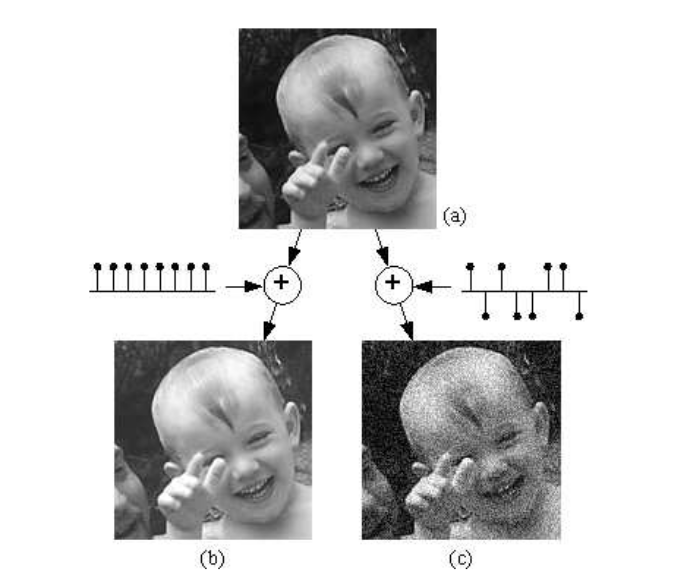
\includegraphics[width=0.5\textwidth]{imagenes/failure_minkowski_metric.png}
  \end{center}
  \caption{En este ejemplo, vemos que sumar una constante positiva a una imágen de 
    referencia (a) produce la imagen (b) que contiene la misma distancia \emph{Minkowski}\footnotemark[1]
  que (c), imagen fabricada por la misma constante pero permutando signo de forma aleatoria. \\\hspace{\textwidth}
\textbf{Créditos}: \emph{The essential guide to Image processing}~\cite{MinkowskiFailure}}
  \label{fig:FailureMinkowskiMetric}
\end{figure}
\begin{figure}[H]
  \begin{center}
    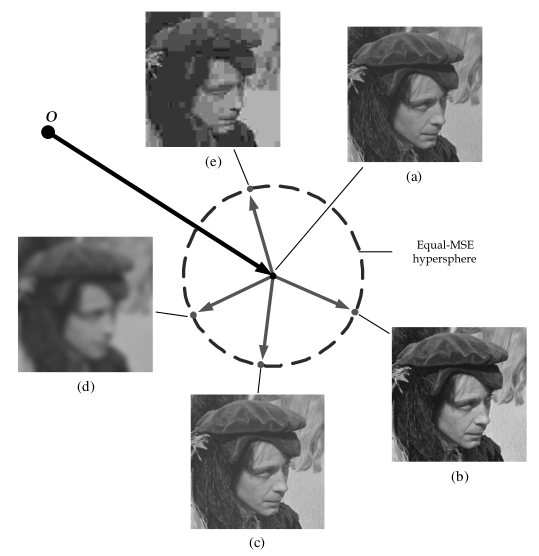
\includegraphics[width=0.5\textwidth]{imagenes/MSE_Hypersphere.png}
  \end{center}
  \caption{En este ejemplo, la misma imágen distorsionada de distinta manera 
  resulta en el mismo valor \emph{MSE}\footnotemark[2]=181. \\\hspace{\textwidth}
  \textbf{Créditos}: Zhou Wang and Alan Conrad Bovik~\cite{Wang2006ModernIQ}}
  \label{fig:MSEHyperSphere}
\end{figure}

\footnotetext[1]{La distancia de \emph{Minkowski} es una métrica en un espacio 
vectorial normalizado que puede considerarse como una generalización tanto de 
la distancia euclidiana como de la distancia de Manhattan . }
\footnotetext[2]{\emph{MSE}: \emph{Mean squared error} o error cuadrático medio 
  es una métrica de distancia que se calcula como la media de la suma de las 
  diferencias al cuadrado.}

\section{Motivación}
\par 
En el caso del ámbito biomédico, dado los rápidos avances en las últimas década
de las técnicas no invasivas de imágenes y la gran cantidad de fabricantes 
de equipamentos, nació el estándar \emph{DICOM}~\cite{Parisot1995} en 1995 
con objetivo de hacer que el intercambio de imágenes médicas se realice de forma 
fácil, segura y con alta calidad. Permitiendo integración con diversos sistemas e 
incluso almacenar información extra en forma de metadatos y anotaciones, así como segmentaciones.
\par 
\missingfigure[figwidth=10cm]{Ejemplos de estructura DICOM + Visualización Slicer}
\par 
A pesar de ello, las distorsiones, que son una ocurrencia común en las imágenes cotidianas, 
están muy presentes en las imágenes médicas~\cite{MedicalImpactOfDistortions}.
Prevalecen las distortiones de contraste, ruido\footnotemark[3] y difuminado.
Estas a su vez, podrían afectar al volúmen 3D que se puede generar a partir 
las imágenes médicas.
\towrite[caption={Continuar Motivacion}]{
  Hablar del uso de modelos 3D para diagnóstico y evaluación y ejemplos de como 
  pueden afectar las distorsiones
}
\section{Objetivos}
\towrite[caption={Objetivos}]{
  Hablar del esquema secuencial que hemos seguido: 
  \par 
  1. Plantear la resolubilidad con uso de caracteríticas NSS (Natural scene 
  statistics) y modelos de aprendizaje automático como SVR, KNNRegressor, Ridge y Tree Regressor. 
  2. Analizar la necesidad del uso de modelos de aprendizaje profundo. (A juego con lo anterior) 
  \par 
  Con ello, el objetivo principal sería algo del estilo: Contribuir a la 
  creación de una métrica de nivel de calidad de imágenes 3D automática,
  acorde con el HVS (Human vision system), y con alto rendimiento para 
  las distorsiones presentes en este ámbito. Generar y demonstrar 
  la posiblidad de generar datasets sintéticos para resolver este problema. 
  Destacando que usaremos uno de partida, el LS-SJTU-PCQA. 
}
\section{Planificación del proyecto}
\towrite[caption={Planificación de Proyecto}]{
    Aquí lo que haría sería un diagrama de Gantt con la planificación 
    desde el mes de febrero. Donde las primeras semanas sería apenas 
    de lectura de artículos y evaluación del estado de arte y posiblidades.
    \par 
    Luego las siguientes semanas serían algo de estilo de implemetanción 
    del modelo sencillo, implementación del modelo NSS complejo (Descomposición 
    del vecindario de los puntos en valores singulares para calcular componentes 
    como esfericidad, planaridad...), implementación del modelo DL, 
    luego implementación de mejoras sobre ambos. 
    \par 
    Hablaría de los saltos que he hecho entre ML con NSS, a DL a ML NSS,
    las pausas, más lecturas y vueltas a implementar más y otras mejoras.
    \par 
    Por último, pondría el análisis de resultados y comienzo de escritura de 
    este documento. Pensaba utilizar el esquema de agrupación que utilizó 
    Valentino en el diagrama de Gantt.
    \par 
    Para terminar este apartado lo que haría sería un presupuesto suponiendo 
    haber trabajado X horas al día durante los días laborales con un salario Y.
    Calcular las horas, multiplicar y asumir otros gastos aparte como lo son 
    el portátil, colab y otros. 
}
